\documentclass[11pt,a4paper]{report}

%load any additional packages
\usepackage{amssymb}
\usepackage{amsmath}
\usepackage{color, soul}
\usepackage{graphicx}
\usepackage{hyperref}
\usepackage{listings}
\usepackage{mathtools}
\usepackage{xcolor}

\newcommand{\defeq}{\vcentcolon=}

\graphicspath{ {./images/} }

\definecolor{codegreen}{rgb}{0,0.6,0}
\definecolor{codegray}{rgb}{0.5,0.5,0.5}
\definecolor{codepurple}{rgb}{0.58,0,0.82}
\definecolor{backcolour}{rgb}{0.95,0.95,0.92}

\lstdefinestyle{mystyle}{
    backgroundcolor=\color{backcolour},   
    commentstyle=\color{codegreen},
    keywordstyle=\color{magenta},
    numberstyle=\tiny\color{codegray},
    stringstyle=\color{codepurple},
    basicstyle=\ttfamily\footnotesize,
    breakatwhitespace=false,         
    breaklines=true,                 
    captionpos=b,                    
    keepspaces=true,                 
    numbers=left,                    
    numbersep=5pt,                  
    showspaces=false,                
    showstringspaces=false,
    showtabs=false,                  
    tabsize=2
}

\lstset{style=mystyle}

\title{Numerical-solver\\[1ex]     %your thesis title,
        Assignment Report}   %note \\[1ex] is a line break in the title

\author{Hui Jia Farm} 

%end the preamble and start the document
\begin{document}

\baselineskip=18pt plus1pt

%set the number of sectioning levels that get number and appear in the contents
\setcounter{secnumdepth}{3}
\setcounter{tocdepth}{3}


\maketitle                  % create a title page from the preamble info
% \include{abstract}          % include the abstract

\tableofcontents            % generate and include a table of contents
% \listoffigures              % generate and include a list of figures


%now include the files of latex for each of the chapters etc
1. Explain finite difference methods.
2. Derive the numerical methods and their truncation error (show error behaviour).

Methods included:
1. One-step method
    a. Euler's explicit
    b. Euler's implicit
    c. 4-stage Runge-Kutta method
    d. trapezium rule
    remarks: fixed point iteration method included to compute implicit methods
2. Predictor-corrector method
    a. Euler-trapezium method
3. Adaptive method
    a. ode23 method (Matlab)
    b. ode45 method (Matlab)
    
%---------------------------------------------------------------------------------
\chapter{Numerical methods}
\label{chap:numerical-methods}
%---------------------------------------------------------------------------------
In real world problems, ODE systems are frequently used. However, these models cannot be solved analytically. Therefore, the solution has to be estimated by numerical methods. The most popular and simple method is the Euler's method.

Intuitively, the Euler's explicit method tries to estimate the value at the next step following the gradient of the solution at current point. If the step size is sufficiently small, the estimation will be accurate.

An initial value problem, has the general form of 
\begin{align}
    y'&=f(x,y)\\
    y(x_0) &= y_0
\end{align}
for $x \in [x_0, X_M]$.

Notation:
Throughout the report, we will use the following notation.
$y_n$ - numerical approximation of $y(x_n)$
$y(x_n)$ - analytical solution at mesh point $x_n$
$x_n$ - mesh points of defined range, where

\begin{align}
    x_n &= x_0 + nh\\
    h &= \frac{(X_M - x_0)}{N}
\end{align}

for $n = 0,\dots, N$

For the simple Euler's explicit method, 
\begin{equation}
    y_{n+1} = y_n + hf(x_n,y_n)\\
\end{equation}

The implementation is as follows:

\begin{lstlisting}[language=Python]
y_n = [self.initial_value]
x_n = [self.x_min]

# Calculate approximated solution for each mesh point.
for n in range(1, self.mesh_points + 1):
    step = [self.mesh_size * f for f in self.func(x_n[-1], y_n[-1])]
    y_n.append([a + b for a, b in zip(y_n[-1], step)])
    x_n.append(self.x_min + n * self.mesh_size)

return x_n, y_n
\end{lstlisting}
%---------------------------------------------------------------------------------
\chapter{Implementation}
\label{chap:code-implementation}
%---------------------------------------------------------------------------------
\section{Software details}
The numerical methods implemented in this software are classified into three classes: one-step methods, predictor-corrector methods and adaptive methods. The methods included are:
\begin{enumerate}
    \item One-step method
    \begin{itemize}
        \item Euler's explicit method
        \item Euler's implicit method
        \item Trapezium rule method
        \item Four-stage Runge-Kutta method
    \end{itemize}
    \item Predictor-corrector method
    \begin{itemize}
        \item Euler-Trapezoidal method
    \end{itemize}
    \item Adaptive method
    \begin{itemize}
        \item BS23 algorithm
        \item RKF45 algorithm
    \end{itemize}
\end{enumerate}
The code is available on Github via \href{https://github.com/FarmHJ/numerical-solver}{this link}. There are badges displayed on the Github repository to indicate that the code are tested to work on several python versions and operating systems. One of the badges also shows the code coverage of the software, which will be described in details in the section \ref{sec:testing}. Finally, there is a status badge to verify that the documentation of the software is built successfully. The documentation of the software can be found \href{https://numerical-solver.readthedocs.io/en/latest/index.html}{here}. 


\includegraphics[width=0.95\columnwidth]{badges}

\section{Unit testing}
\label{sec:testing}
In the progress of constructing the software, a unit testing infrastructure was put in place. The purpose of the unit testing is to create a robust and sustainable software. Written codes are tested to make sure it runs as intended and returns expected results. If code is tested while writing, it would be easier to fix bugs in the future as previously tested code would be correct and most probably free of bugs. Code coverage is used to define the percentage of codes covered in the unit testing process. It is usually aim to achieve a 100\% code coverage. However, a 100\% code coverage does not necessarily mean that the code is correct or free of errors. Nevertheless, it provides some confidence that the code is implemented correctly.

Every method in this numerical-solver software is tested. The numerical solution of each method is tested to give the same solution as a manually calculated solution. The methods are mostly tested against the example model \ref{eqn:example_model}.

\section{Testing initialisation}
The initialisations of each class are tested to ensure that variables are initialised correctly and input type satisfies the requirements. For example, 

\begin{lstlisting}[language=Python]
def test__init__(self):

    def func(x, y):
        return [-y[0]]
    x_min = 0
    x_max = 1
    initial_value = [1]
    mesh_points = 10

    problem = solver.OneStepMethods(
        func, x_min, x_max, initial_value, mesh_points)

    # Test initialisation
    self.assertEqual(problem.x_min, 0)
    self.assertEqual(problem.mesh_points, 10)

    # Test raised error for callable function
    with self.assertRaises(TypeError):
        solver.OneStepMethods(
            x_min, x_min, x_max, initial_value, mesh_points)

    # Test raised error if initial_value not list
    with self.assertRaises(TypeError):
        solver.OneStepMethods(
            func, x_min, x_max, 1, mesh_points)
\end{lstlisting}
. A simple model with analytical solution is first initialised. Required inputs were check to make sure the problem is set up properly, in line 14 and 15 of the code snippet above. To ensure that the inputs to the function are of the desired data type, errors are raised whenever the user inputs a wrong data type. The unit testing also tests that these errors are raised appropriately (line 17 to 25) whenever the data type does not satisfy the requirements. 

\section{Testing function}
After checking that the problem is properly initialised, we then test that the numerical methods are working correctly. Take the adaptive method, BS23 algorithm, as an example, 
\begin{lstlisting}[language=Python]
def test_ode23(self):

def func(x, y):
    return [-y[0]]
x_min = 0
x_max = 1
initial_value = [1]

problem = solver.AdaptiveMethod(
    func, x_min, x_max, initial_value, initial_mesh=0.5)
mesh, soln = problem.ode23()

# Test end point of mesh
self.assertGreaterEqual(mesh[-1], 1.0)

# Test mesh point
self.assertAlmostEqual(mesh[1], 0.3483788976565)

# Test solution at first stepsize
self.assertAlmostEqual(soln[1][0], 0.7052580305097)
\end{lstlisting}
The method is first tested to execute the numerical computation up to the maximum mesh point indicated. Then the first adaptive mesh point and its solution, obtained from the software, matches the value computed manually. 
%---------------------------------------------------------------------------------
\chapter{Fitzhugh-Nagumo Model Example}
\label{chap:fitzhugh-nagumo}
%---------------------------------------------------------------------------------
\section{Background}
\label{sec:background}
% reference from brugada symdrome essay and keener sneyd
We will look into the Fitzhugh-Nagumo model in this assignment. The Fitzhugh-Nagumo model is a model that describes an excitable system, such as the action potential of cardiac cells. The action potential is first described by Hodgkin \& Huxley. Their model were then simplified to the Fitzhugh-Nagumo model, retaining the fast-slow phase and excitability of the Hodgkin \& Huxley model. %\ref{cite:keener&sneyd}

\section{Fitzhugh-Nagumo model}
\label{sec:FHN}
The definition of the Fitzhugh-Nagumo model is
\begin{align}
    \epsilon \frac{dv}{dt} &= f(v) - w + \mathbf{I}_{app} \\
    \frac{dw}{dt} &= v - \gamma w
\end{align}
where $f(v) = v(1-v)(v-\alpha)$, $0 < \alpha < 1$, $\epsilon \ll 1$ and $\mathbf{I}_{app}$ is the applied current. The fast $v$ is the excitation variable, while the slow $w$ is the recovery variable.

In this implementation, the parameters are chosen to be $\alpha = 0.1$, $\gamma = 0.5$, $\epsilon = 0.01$ and $\mathbf{I}_{app} = 0.026$, taking reference from %\ref{cite:appadu}
The initial values are taken to be near the origin, that are $(v_0, w_0) = (0.01, 0.01)$. 

The Fitzhugh-Nagumo is solved with various numerical methods in this \href{https://nbviewer.jupyter.org/github/FarmHJ/numerical-solver/blob/main/examples/fitzhugh_nagumo.ipynb}{Fitzhugh-Nagumo solution notebook}. 

\begin{figure}
    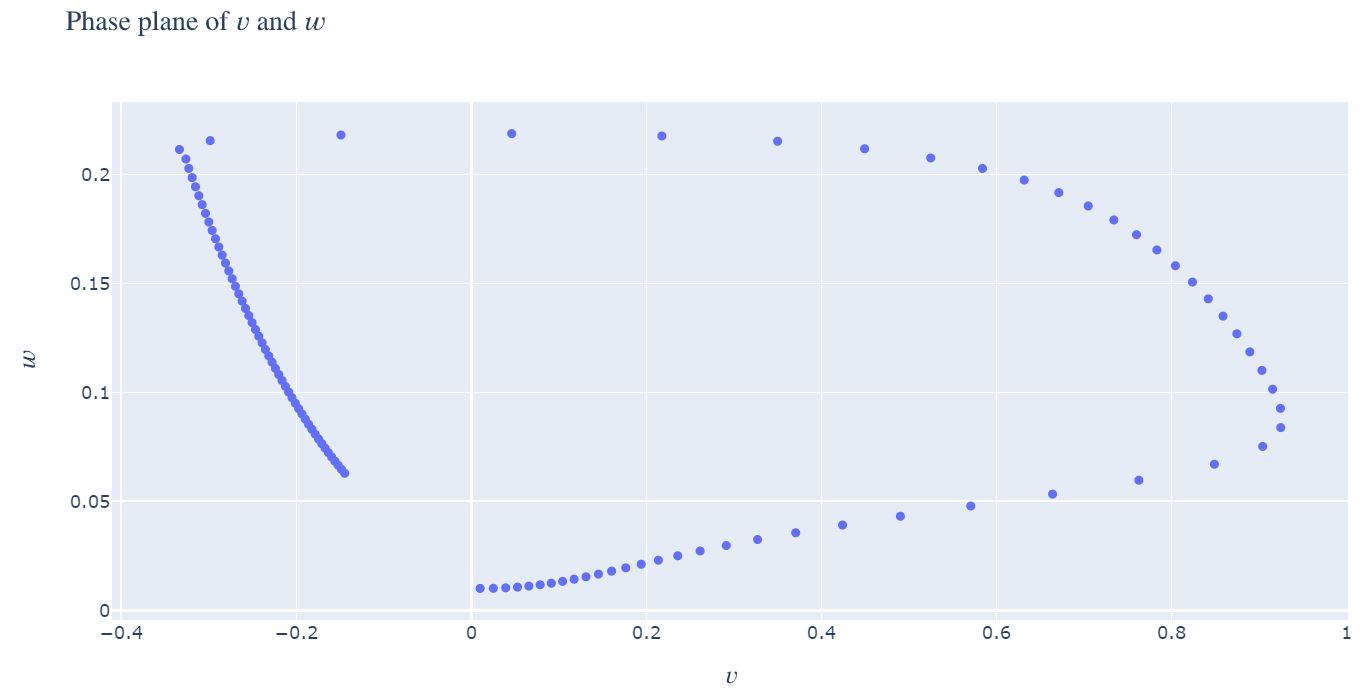
\includegraphics[width=0.95\columnwidth]{FHN_Euler_explicit_phase_plane}
    \caption{Phase plane of $v$ and $w$ by Euler's explicit method.}
    \label{fig:Euler_explicit_phase_plane}
\end{figure}

\begin{figure}
    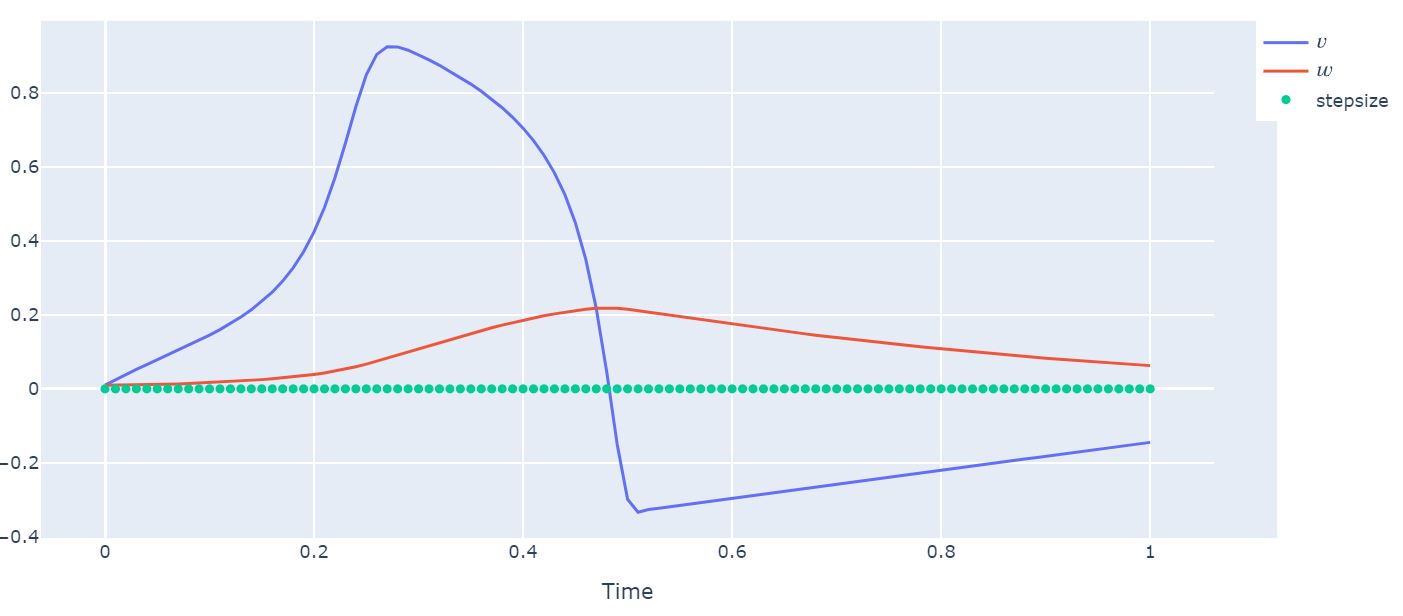
\includegraphics[width=0.95\columnwidth]{FHN_Euler_explicit_variable}
    \caption{Graph of $v$ and $w$ against time by Euler's explicit method.}
    \label{fig:Euler_explicit_variable}
\end{figure}


From the figure \ref{fig:Euler_explicit_variable}, we can see that $v$, the excitation variable is excited in the early stage. While $v$ increases significantly, the change in $w$ is small. After $v$ reaches its peak and starts to reduce, $w$ increases slowly. This can be observed in both phase plane (Fig. \ref{fig:Euler_explicit_phase_plane}) and variable graph (Fig. \ref{fig:Euler_explicit_variable}). When the variable $v$ starts to recover to its original value, $w$ is at its maximum. The scattering of points in the phase plane captures the feature of the model, where the change in $v$ is rapid while the change in $w$ is slow. When the change in $v$ is significantly larger than the change in $w$, the points are sparse. On the other hand, the points are packed when $w$ increases or decreases more than $v$. However, in the adaptive methods, such insights cannot be interpreted directly from the phase plane. Therefore, green triangles were plotted in Fig. \ref{fig:adaptive_variable} to indicate the adapted mesh points. The mesh points are adapted towards large difference in $v$ or $w$ over a short period of time.

\begin{figure}
    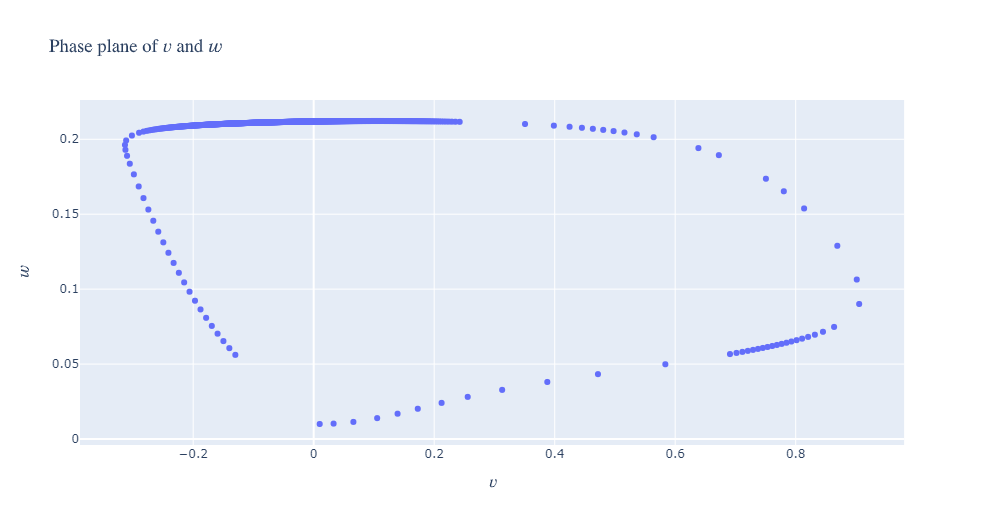
\includegraphics[width=0.95\columnwidth]{FHN_adaptive_phase_plane}
    \caption{Phase plane of $v$ and $w$ for adaptive method BS23.}
    \label{fig:adaptive_phase_plane}
\end{figure}

\begin{figure}
    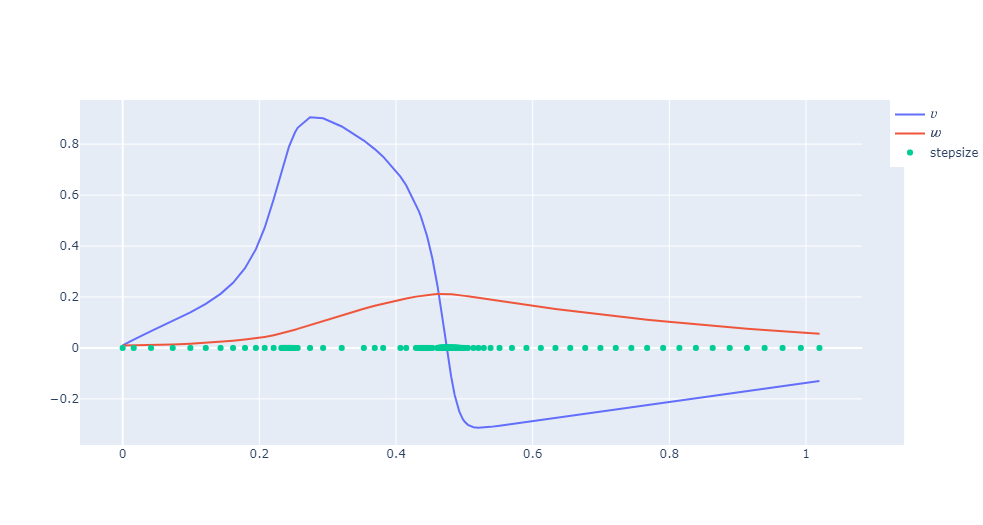
\includegraphics[width=0.95\columnwidth]{FHN_adaptive_variable}
    \caption{Graph of $v$ and $w$ against time for adaptive method BS23}
    \label{fig:adaptive_variable}
\end{figure}

\section{Convergence of Fitzhugh-Nagumo model}
\label{sec:FHN-convergence}
A \href{https://nbviewer.jupyter.org/github/FarmHJ/numerical-solver/blob/main/examples/fhn_model_convergence.ipynb}{notebook} is created to test the convergence of the solution to the Fitzhugh-Nagumo model. Since the model has no analytical solution, it is tested against a reference solution. The reference solutions are assumed to be sufficiently accurate. For methods with fixed step size, which are the one-step methods and predictor-corrector method, the reference solutions are constructed by using smaller step size. For methods with adaptive step size, reference solutions are obtained by using smaller tolerance value. This notebook shows the numerical solution computed for different methods at different step sizes or tolerance values. The numerical solutions are then compared with their respective reference solutions. In both methods, the error decreases as step size or tolerance decreases.

\begin{figure}
    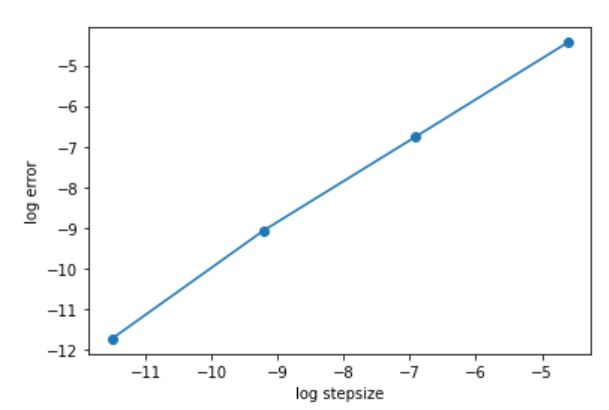
\includegraphics[width=0.95\columnwidth]{FHN_Euler_explicit_error_behaviour}
    \caption{Error at a mesh point for Euler's explicit method.}
    \label{fig:Euler_explicit_error}
 \end{figure}
\begin{figure}
   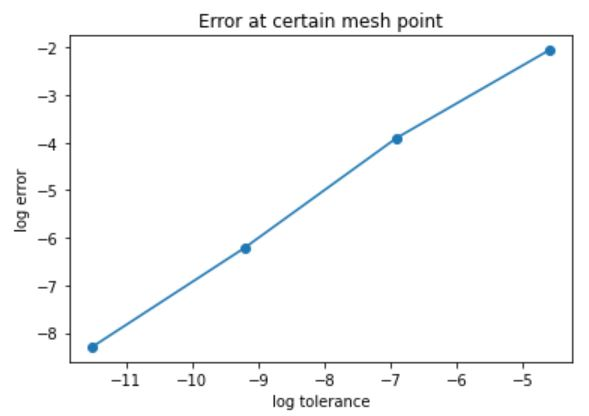
\includegraphics[width=0.95\columnwidth]{FHN_adaptive_error_behaviour}
   \caption{Sum of error for adaptive method BS23.}
   \label{fig:adaptive_error}
\end{figure}

%now enable appendix numbering format and include any appendices
% \appendix
% \include{appendix1}
% \include{appendix2}

%next line adds the Bibliography to the contents page
% \addcontentsline{toc}{chapter}{Bibliography}
%uncomment next line to change bibliography name to references
%\renewcommand{\bibname}{References}
% \bibliography{refs}        %use a bibtex bibliography file refs.bib
% \bibliographystyle{plain}  %use the plain bibliography style

\end{document}